\section{Electrical Power Systems}
\subsection{EPS Scheme}

The figure \ref{epsbasics} shows how the different electrical subsystems are related with one another.

\begin{figure}[H]
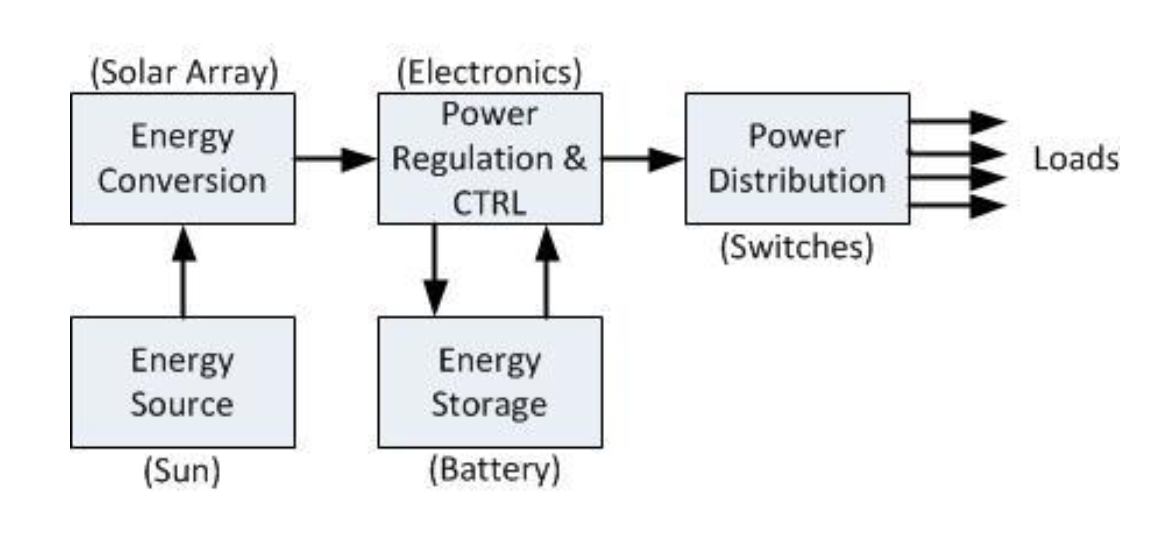
\includegraphics[scale=0.6]{./sections/SatelliteDept/sections/images/epsbasics}
\centering
\caption[Basic schematics of the EPS]{Basic schematics of the EPS. Source \cite{epsbasics}} 
\label{epsbasics}
\end{figure}

The need for a system that regulates, manages and distributes the energy to all of the other subsystems is clear. Every system (or load) has its own energy needs and the power distributing system must have several buses in order to maintain all the systems working at the same time. Also, redundant buses and connections should be mounted to ensure the least possible failures in the EPS; a failure of the EPS could compromise the whole satellite.

The electrical power unit should also measure the power consumed in real time and the intensity and voltage of the different buses to communicate possible failures to the on-board computer. If a failure is detected, the system should adapt in order to avoid being \textit{in the dark} (this is: there has to be some power always available).

\subsection{Estimation of the power required}
The vast majority of the time, the subsystems of the satellite will work under typical operation conditions. However, the estimation of the power consumption provided in the table \ref{powerestimation} has been made for \textit~{typical-high} conditions in order to have a power margin and a more reliable estimation.

\pagebreak
\begin{longtable}{| l | r | }
\hline
\rowcolor[gray]{0.80}	\textbf{System (number of units)} &  \textbf{Typical power consumption per unit (W)} \\
\hline
\endfirsthead

\rowcolor[gray]{0.85} \textbf{Payload} &  \\
	   ~Patch antenna (8) & 4 \\
	   \rowcolor[gray]{0.95} \textbf{Payload power consumption} & 32 \\
	   \hline
	\hline

\rowcolor[gray]{0.85} \textbf{Electrical Power System} &  \\
	   ~NanoPower P60 Power Module (1) & 2 \\
	   ~Battery (2) & - \\
	   ~Solar arrays (4) & -\\
	   \rowcolor[gray]{0.95} \textbf{EPS power consumption} & 2 \\
	   \hline
	\hline
	
\rowcolor[gray]{0.85} \textbf{Data Handling Systems} &  \\
	   ~Transceiver inner-satellite (3) & 4 \\
	   ~Transceiver space to ground (1) & 4 \\
	   ~Data handling system (1) & 4 \\
	   \rowcolor[gray]{0.95} \textbf{DHS power consumption} & 15 \\
	   \hline
	\hline
	
\rowcolor[gray]{0.85} \textbf{Propulsion and ACDS} &  \\
	   ~Thruster (1) & 20 \\
	   ~ADACS (1) & 3 \\
	   \rowcolor[gray]{0.95} \textbf{OACDS power consumption} & 3 \\
	   \hline
	\hline

\rowcolor[gray]{0.65} \textbf{Estimated total power consumption} & 52 \\

\caption{Estimation of the power consumption under typical working conditions}
\label{powerestimation}
\end{longtable}

It is worth mentioning that the thrusters are not included in the final estimation of the power. The propulsion system will only be active for shorts periods of time to maintain the orbit, and when it ignites, the other subsystems will not perform under typical working conditions. The CubeSat will manage to send only the essential information to the other satellites and, since it is unlikely that their thruster is ignited at the same time, the communication is ensured during the maneuver. There will not be any loss of communication given the different ground stations placed around the Earth and the capacity of the satellite to communicate the essential information to its constellation neighbours.

\subsection{Solar arrays}
They are an essential part of the mission since they are the main source of energy for the CubeSat. The solar arrays used must have a decent efficiency and capacity to collect the energy from the sun, have to keep their mass relatively low, must have a protective radiation shield to ensure their full efficiency for at least 4 years, a proper deployment system, the ability to withstand space conditions and also must be highly compatible with all the other systems used, especially the power management system.

Two options were considered regarding the solar arrays. These options are presented in \ref{solararraysoptions}.

\begin{longtable}{| l | c | c | }
\hline
\rowcolor[gray]{0.80}	\textbf{Brand and model} &  \textbf{Features}     & \textbf{Total price (\euro) per unit}   \\
\hline
\endfirsthead

\rowcolor[gray]{0.85} \textbf{Solar arrays} &  &  \\
	   ~EXA-Agencia Espacial Ecuatoriana & \makecell{Total power of 67.2W (4 units)\\ Mass of 175g (per unit) \\ Included thermal protection \\At least 4 years lifetime} & 17000 \\
	   \hline
	   ~ISIS & \makecell{Total power of ~30W (4 units) \\ Mass of 150g (per unit) \\ No thermal protection \\At least 2 years lifetime} & 9000 \\
	   \hline
\caption{Options studied for the solar arrays}
\label{solararraysoptions}
\end{longtable}

The option selected for the mission is a set of deployable solar panels provided by \textbf{EXA (Agencia Espacial Civil Ecuatoriana)}. These solar arrays fulfill all the requirements mentioned above: they are low mass (135g per unit + 40g of cable weight), they have a protective radiation shield (NEMEA Anti Radiation Shield protects the solar panels of EM, High Gamma, X-Ray, Alfa, Beta and low neutron radiation) they can withstand a very high temperature range (from -80ºC to 130ºC) ensuring that they can operate in space, they have a gentle release and deployment system with artificial muscles (developed by EXA) and they provide a power of 16.8W each (19.2V@0.5A).

Every CubeSat will come with at least 4 deployable solar panels providing it with 67.2W of power, approximately. Note that additional panels can be equipped but they have to be also low mass equipment (about 80g per array) and highly compatible with the structure of the CubeSat.

\subsection{Power management system}
From the figure \ref{epsbasics}, the need of a system that regulates and distributes the energy to the other systems is more than clear. In fact, the  Power Management System (PMS) is mandatory for this CubeSat given that the systems used are manufactured by different companies and they have completely different specifications regarding its energy requirements.

Several options were considered regarding the power management system. These options, with their respective main features, are presented in \ref{optionspowermanagementsystem}.

\pagebreak
\begin{longtable}{| l | c | c | }
\hline
\rowcolor[gray]{0.80}	\textbf{Brand and model} &  \textbf{Features}     & \textbf{Total price (\euro) per unit}   \\
\hline
\endfirsthead
\rowcolor[gray]{0.85} \textbf{Power management} &  &  \\
	   ~Crystalspace P1 Vasik & \makecell{Mass of 80g \\ Full redundancy \\ Low volume \\ 6x outputs \\ Up to 10W input \\ High temperature range} & 5400 \\
	\hline
	   ~Gomspace NanoPower P60 & \makecell{Mass of 176g \\ 9x configurable outputs \\ 6x inputs per module \\ EMI shielding \\ High temperature range} & 16000 \\
	\hline
\caption{Options studied for the power management system}
\label{optionspowermanagementsystem}
\end{longtable}

The selected option for the mission is the \textbf{NanoPower P60} by \textbf{Gomspace}, a high-power EPS for small satellites that comes with 1 motherboard, 1 ACU module (Array Conditioning Unit) and 1 PDU (Power Distribution Unit), allowing multiple configurations in just one motherboard; saving a lot of space.

The motherboard supports up to 4 ACU and PDU modules and has different regulated outputs (3.3V and 5V). It means that with one single motherboard, several conditioning and distributing units can be connected. That ensures that additional equipment (ACU and PDU) could be linked to the motherboard if something failed in the assembly process.

The ACU module 6 different inputs per unit with a high voltage solar input (up to 16V or 32V). Additionally, each input can withstand a maximum current of 2A and current and voltage inputs are measured on each input channel and the measurements can be communicated to the on board computer.

The PDU module has 9 different outputs per unit that are highly configurable. Each module has 3 configurable output voltages (3.3V, 5V, 8V, 12V, 18V, 24V) and each of the outputs can withstand a maximum current of 1A or 2A (programmable). Additionally, like the ACU module, current and voltage outputs are measured on each output channel and can be effectively communicated to the on board computer.

All these features make the \textbf{NanoPower P60} a very efficient and configurable power management unit that fulfills the mission requirements. Furthermore, given this capacity to configure each input and output channel and the high number of channels that it has, the compatibility between all the systems used in the satellite is ensured. Additionally, the communication between this system and the on board computer in order to detect potential failures is a really adequate feature, mentioned previously.\\
With the NanoPower P60, the PMS aims to distribute the energy to all of the subsystems of the CubeSat.

\subsection{Batteries}

The batteries have to provide the energy that the system requires when the solar arrays are not operational. Therefore, it is a very important system due to an energy loss could mean a mission failure (although it would be unlikely since more CubeSats would be ready to handle the information of the CubeSat that failed). The following options (\ref{optionsbatteries}) were considered.

\begin{longtable}{| l | c | c | }
\hline
\rowcolor[gray]{0.80}	\textbf{Brand and model} &  \textbf{Features}     & \textbf{Total price (\euro) per unit}   \\
\hline
\endfirsthead
\rowcolor[gray]{0.85} \textbf{Batteries} &  &  \\
	   ~Gomspace NanoPower BP4 & \makecell{Total capacity of 77Wh (2u) \\ Automatic heat regulation \\ Highly stackable \\ Mass of 270g (p.unit)} & 3250 \\
	\hline
	~EXA-Agencia Espacial Ecuatoriana & \makecell{Total capacity of 106.4Wh (2u)\\ Automatic heat regulation \\ Highly stackable \\ Total mass of 155g} & 6300 \\
	\hline
	
\caption{Options studied for the batteries}
\label{optionsbatteries}
\end{longtable}

Astrea has chosen the \textbf{BA01/D} batteries manufactured by \textbf{EXA-Agencia Espacial Civil Ecuatoriana}. The CubeSat will have two of these batteries, with a total capacity of 28800mAh or 106,4Wh. Each battery has a total of 16 cells, highly stackable and with a very low mass (155g per unit). They also come with unique thermal transfer bus, that will transfer the heat of the other subsystems to the batteries to keep their temperature under efficient working conditions.

The output voltage can be configured (3.7V and 7.4V) and they are perfectly compatible with the solar arrays. Furthermore, they come with a protective radiation shield (NEMEA) that ensures at least 4 years working under full efficiency conditions in a LEO. It is also worth mentioning that if the company that will assemble the CubeSat faces problems during this part of the process, the batteries can be customized by contacting EXA.

As mentioned above, if the satellite was in the dark during half of the period of the orbit, the estimated energy that it would need would be ~50W. Thereby, the capacity of the batteries is more than enough to supply the required energy in the worst case scenario. In fact, they will supply energy when the energy demand of the CubeSat is higher than the energy collected by the solar cells. And logically, they will store the energy collected by the solar arrays when the energy demand of the systems is lower than the energy collected.